%%% 数学コンテンツ %%%

\documentclass[dvipdfmx]{jsarticle}
\usepackage[top=20truemm, bottom=20truemm, left=20truemm, right=20truemm]{geometry}
\usepackage{amsmath, amssymb, amsthm}
\usepackage{mathtools}
\usepackage[dvipdfmx]{graphicx}
\usepackage{framed}
\usepackage{url}
\usepackage{comment}
\usepackage[dvipdfmx]{hyperref}
\usepackage{pxjahyper}

\theoremstyle{definition}
\newtheorem{definition}{定義}[section]
\newtheorem{theorem}[definition]{定理}
\newtheorem{example}[definition]{例}
\newtheorem{question}{問}[section]


\title{鑑賞するフラクタル}
\author{吉永 塁 \thanks{情報工学課程4年 \texttt{b7122062@edu.kit.ac.jp}}}
\date{\today}

\begin{document}

\maketitle{}



%%% ===============================================================================
\section{はじめに}

問題を解いたり証明を考えたりするだけでなく,「鑑賞」するのも数学との向き合い方の一つとしてあっても良いのではないかと思います.
題材としてフラクタルとセルオートマトンを取り上げます.
理論的な厳密さは不十分かもしれませんが,自分が書いたコードによって図形が実際に描かれていく楽しさを感じてもらえればと思います.
ソースコードは後ろのページに付録として掲載しました.
実際に動かしてみたり,改良したりして遊んでいただければと思います.


%%% ========================================================
\subsection{Processingについて}

今回,図形を描くのにProcessingを用います.
Processingは,Javaをベースとしたグラフィクスに特化したプログラミング言語です.
比較的短い記述で簡単に図形を描くことができるのが特徴です.
煩雑なことをせずに視覚的な出力が得られるので,プログラミングに馴染のない方でも親しみやすいかと思います.
コード例は全てProcessingで記述されていますが,他の言語で使い馴染んだものがあるならば,そちらを使っていただいても構いません.

注意事項として,Processingの座標は原点が左上で$y$軸が下向き正として取られていることに気を付けてください.
その他の構文や関数などについて,詳しくは\cite{pcweb}を参照していただければと思います.
また,Processing全般についての書籍として,\cite{genart},\cite{cgmediaart}が参考になるかと思います.
その他にも,\cite{mathgen}では,数学を題材として取り上げています.



%%% ===============================================================================
\section{フラクタル・再帰}

フラクタル図形とは,図形の一部が全体の相似形となっているような図形のことをいいます.

また,ある関数定義の中で,その関数自身を呼び出すような構造を持つ関数のことを再帰関数と呼びます.

この章では再帰関数によってフラクタル図形を描いていきます.


%%% ========================================================
\subsection{Sierpinskiのカーペット}
\label{subsec_carpet}

Sierpinskiのカーペットとは,図\ref{pic_carpet}のような,正方形の中心を取り除くという操作を繰り返すことで得られるフラクタル図形です.

\begin{figure}[ht]
\begin{center}
    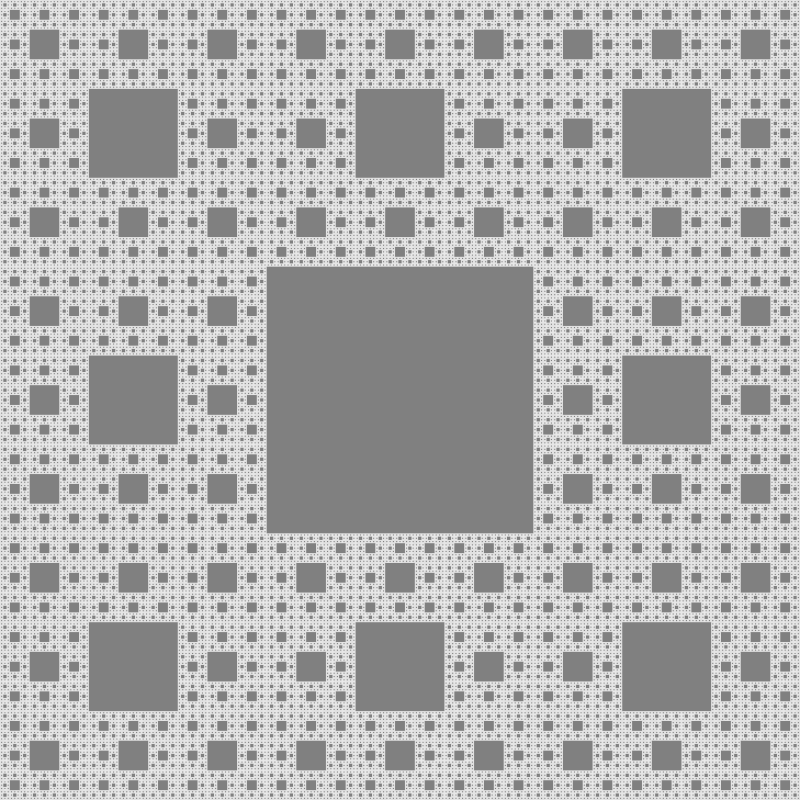
\includegraphics[scale=0.15]{figure/carpet.png}
\end{center}
\caption{Sierpinskiのカーペット}
\label{pic_carpet}
\end{figure}

Sierpinskiのカーペットをプログラムで描く方法を考えます.
Sierpinskiのカーペットは次の規則によって得られます.
\begin{enumerate}
    \item 与えられた正方形を$3 \times 3$の小正方形に分割する. \label{alg_carpet_fst}
    \item 分割してできた9個の小正方形のうち,中心にあるものを取り除く.
    \item 残りの8個の小正方形を\ref{alg_carpet_fst}の正方形として同様の操作を繰り返す.
    \item これらの操作を適当な回数繰り返す.
\end{enumerate}

この操作を再帰関数として記述すると図\ref{code_carpet}のようになります.

プログラム全体は\ref{code_carpet_all}節に記載しました.
出力は図\ref{pic_carpet}のようになります.

\begin{figure}[ht]
\begin{center}
\begin{oframed}
\footnotesize
\begin{verbatim}
    void carpet(float x, float y, float l, int n) {

        if( n <= 0 ){
            return ;
        }

        float sqlen = l / 3;  // 小正方形の辺の長さ

        square(x+sqlen, y+sqlen, sqlen);  // 中心

        carpet(x        , y        , sqlen, n-1);  // 上左
        carpet(x+sqlen  , y        , sqlen, n-1);  // 上中
        carpet(x+2*sqlen, y        , sqlen, n-1);  // 上右
        carpet(x        , y+sqlen  , sqlen, n-1);  // 中左
        carpet(x+2*sqlen, y+sqlen  , sqlen, n-1);  // 中右
        carpet(x        , y+2*sqlen, sqlen, n-1);  // 下左
        carpet(x+sqlen  , y+2*sqlen, sqlen, n-1);  // 下中
        carpet(x+2*sqlen, y+2*sqlen, sqlen, n-1);  // 下右

        return ;
    }
\end{verbatim}
\end{oframed}
\end{center}
\caption{Sierpinskiのカーペットを描く再帰関数}
\label{code_carpet}
\end{figure}

また,Sierpinskiのカーペットを3次元の立体へ拡張したものはMengerのスポンジと呼ばれます.


%%% ========================================================
\subsection{Sierpinskiのギャスケット}

Sierpinskiのギャスケットとは,図\ref{pic_gasket}のような,三角形の中心を取り除く操作を繰り返すことで得られるフラクタル図形です.
\ref{subsec_carpet}節でみたSierpinskiのカーペットの三角形版です.

\begin{figure}
\begin{center}
    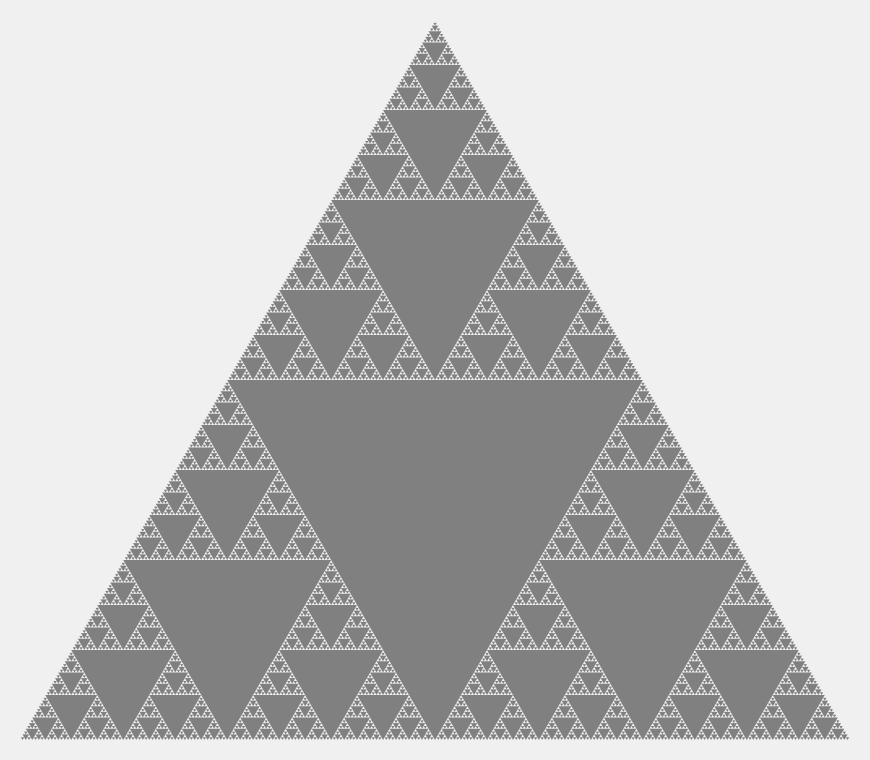
\includegraphics[scale=0.20]{figure/gasket.png}
\end{center}
\caption{Sierpinskiのギャスケット}
\label{pic_gasket}
\end{figure}

Sierpinskiのギャスケットは,Sierpinskiのカーペットとほぼ同様にして得られます.
Sierpinskiのカーペットを得る手順において,正方形を正三角形に置き換えるだけです.

Sierpinskiのカーペットを描く再帰関数は図\ref{code_gasket}のようになります.

プログラム全体は\ref{code_gasket_all}節に記載しました.
出力は図\ref{pic_gasket}のようになります.

\begin{figure}
\begin{center}
\begin{oframed}
\footnotesize
\begin{verbatim}
    void gasket(float tx, float ty, float lx, float ly, float rx, float ry, int n) {

        if ( n <= 0 ) {
            return ;
        }

        float lcx = (tx + lx) / 2;  // 上頂点と左頂点の中間点のx座標
        float lcy = (ty + ly) / 2;  // 上頂点と左頂点の中間点のy座標
        float rcx = (tx + rx) / 2;  // 上頂点と右頂点の中間点のx座標
        float rcy = (ty + ry) / 2;  // 上頂点と右頂点の中間点のy座標
        float bcx = (lx + rx) / 2;  // 左頂点と右頂点の中間点のx座標
        float bcy = (ly + ry) / 2;  // 左頂点と右頂点の中間点のy座標

        triangle(lcx, lcy, rcx, rcy, bcx, bcy);  // 中心

        gasket(tx , ty , lcx, lcy, rcx, rcy, n-1);  // 上
        gasket(lcx, lcy, lx , ly , bcx, bcy, n-1);  // 左
        gasket(rcx, rcy, bcx, bcy, rx , ry , n-1);  // 右

        return ;
    }
\end{verbatim}
\end{oframed}
\end{center}
\caption{Sierpinskiのギャスケットを描く再帰関数}
\label{code_gasket}
\end{figure}


%%% ========================================================
\subsection{高木曲線}

高木曲線とは図\ref{pic_takagi_curve}のような,三角波の足し合わせによって得られるフラクタル図形です.

\begin{figure}
\begin{center}
    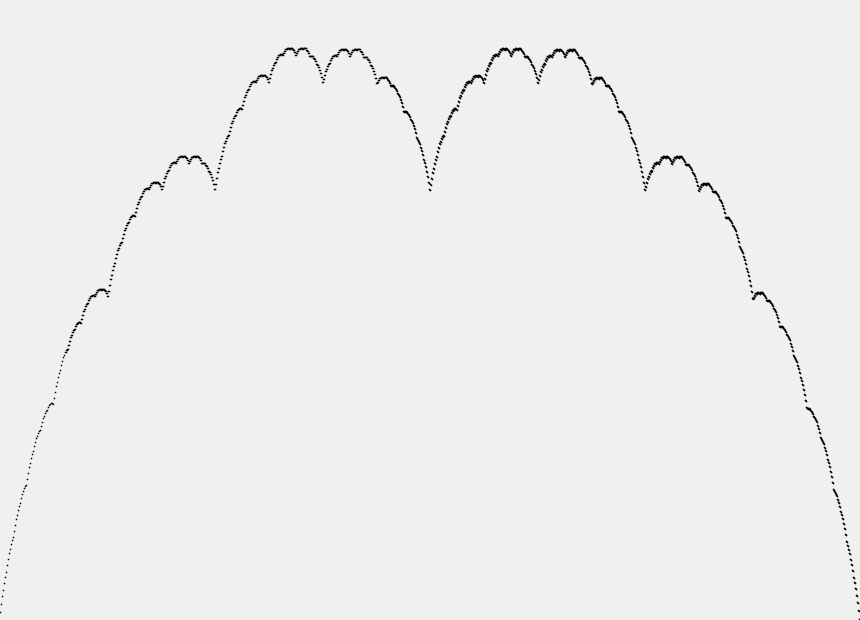
\includegraphics[scale=0.20]{figure/takagi_curve.png}
\end{center}
\caption{高木曲線}
\label{pic_takagi_curve}
\end{figure}

高木曲線は次の規則によって得られます.
\begin{enumerate}
    \item 与えれた区間の中心を頂点とするような三角波を考える. \label{alg_takaki_fst}
    \item 区間を中心で二分割し,左右の小区間を\ref{alg_takaki_fst}の区間として同様の操作を繰り返す.
    \item これらの操作を適当な回数繰り返す. \label{alg_takaki_lst}
    \item 各点について,\ref{alg_takaki_fst}から\ref{alg_takaki_lst}の手順で得られた全ての三角波の高さを足し合わせる.
\end{enumerate}

この操作を再帰関数として記述すると図\ref{code_takagi_curve}のようになります.

プログラム全体は\ref{code_takagi_curve_all}節に記載しました.
出力は図\ref{pic_takagi_curve}のようになります.

\begin{figure}[ht]
\begin{center}
\begin{oframed}
\footnotesize
\begin{verbatim}
    void tcurve(int lx, int rx, int n) {

        if( n <= 0 ){
            return ;
        }

        int cx = (lx + rx) / 2;  // 区間の中心点
        int y = 0;               // 三角波の高さ

        for ( int x = lx; x < cx; x++ ) {
            ys[x] += y++;
        }
        for ( int x = cx; x < rx; x++ ) {
            ys[x] += y--;
        }

        tcurve(lx, cx, n-1);  // 左
        tcurve(cx, rx, n-1);  // 右

        return;
    }
\end{verbatim}
\end{oframed}
\end{center}
\caption{高木曲線を描く再帰関数}
\label{code_takagi_curve}
\end{figure}

% また,高木曲線は次のような関数として表されます.
% \begin{align*}
%     T(x) = \sum_{n=0}^{\infty} \frac{\gamma(2^n x)}{2^n}
% \end{align*}
% ここで$\gamma(x)$は次のように定められる関数です.
% \begin{align*}
%     \gamma(x) = \min_{m \in \mathbb{Z}} |x - m|
% \end{align*}

% この関数$T(x)$は,連続関数でかつ至る所で微分不可能であるという性質を持ちます.
また,高木曲線は特徴として,連続且つ至る所で微分不可能であるという性質を持ちます.


%%% ========================================================
\subsection{Koch曲線}

Koch曲線とは図\ref{pic_koch_curve}のような,線分を三分割し,中央の部分を山形にするという操作を繰り返すことで得られるフラクタル図形です.

\begin{figure}[ht]
\begin{center}
    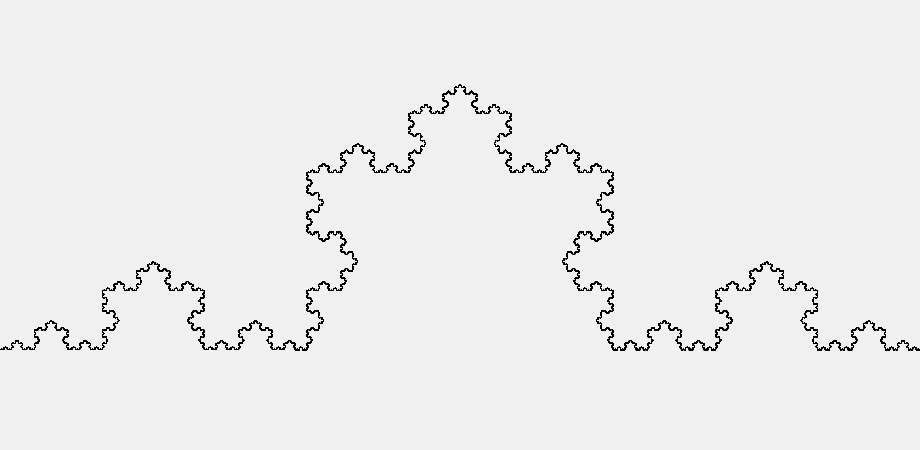
\includegraphics[scale=0.20]{figure/koch_curve.png}
\end{center}
\caption{Koch曲線}
\label{pic_koch_curve}
\end{figure}

Koch曲線は次の規則によって得られます.
\begin{enumerate}
    \item 与えられた線分を3つの小線分に三等分する.  \label{alg_koch_fst}
    \item 中央の小線分を,小線分を一辺とするような正三角形の残りの二辺と置き換える.  \label{alg_koch_snd}
    \item \ref{alg_koch_fst},\ref{alg_koch_snd}でできた4つの小線分を\ref{alg_koch_fst}の線分として同様の操作を繰り返す.
    \item これらの操作を適当な回数繰り返す.
\end{enumerate}

この操作を再帰関数として記述すると図\ref{code_koch_curve}のようになります.

プログラム全体は\ref{code_koch_curve_all}節に記載しました.
出力は図\ref{pic_koch_curve}のようになります.

\begin{figure}[ht]
\begin{center}
\begin{oframed}
\footnotesize
\begin{verbatim}
    void kochcurve(float lx, float ly, float rx, float ry, int n) {

        if ( n <= 0 ) {
            line(lx, ly, rx, ry);
            return ;
        }

        float dx = (rx - lx) / 3;  // 小線分x成分
        float dy = (ry - ly) / 3;  // 小線分y成分
        float cx = (lx + rx) / 2;  // (lx,ly),(rx,ry)の中心x座標
        float cy = (ly + ry) / 2;  // (lx,ly),(rx,ry)の中心y座標

        kochcurve(lx             , ly             , lx+dx          , ly+dy          , n-1);  // 左
        kochcurve(lx+dx          , ly+dy          , cx-sqrt(3)/2*dy, cy+sqrt(3)/2*dx, n-1);  // 中左
        kochcurve(cx-sqrt(3)/2*dy, cy+sqrt(3)/2*dx, rx-dx          , ry-dy          , n-1);  // 中右
        kochcurve(rx-dx          , ry-dy          , rx             , ry             , n-1);  // 右

        return ;
    }
\end{verbatim}
\end{oframed}
\end{center}
\caption{Koch曲線を描く再帰関数}
\label{code_koch_curve}
\end{figure}

Koch曲線も高木曲線と同様,連続且つ至る所で微分不可能であるという性質を持ちます.
また,図\ref{pic_koch_snowflake}の様に,Koch曲線を3つ用いて星形のように繋げた図形をKoch雪片といいます.


\vspace{\baselineskip}

%%% ========================================================
\begin{question}
    Vicsekフラクタル(図\ref{pic_vicfr_x},図\ref{pic_vicfr_c})を描くプログラムを作成してください.
\end{question}

\begin{question}
    Cantor集合(図\ref{pic_cantorset})を描くプログラムを作成してください.
\end{question}

\begin{question}
    Hexaflake(図\ref{pic_hexfr})を描くプログラムを作成してください.
    正六角形の書き方は,図\ref{code_hexfunc}を参考にしてください.
\begin{figure}[ht]
\begin{center}
\footnotesize
\begin{oframed}
\begin{verbatim}
    void hexagon(float x, float y, float l) {

        /* (x,y)を中心とする頂点までの長さがlの正六角形 */
        beginShape();
        for ( float t = 0; t < TWO_PI; t += TWO_PI/6 ) {
            vertex(x+l*cos(t), y+l*sin(t));
        }
        endShape(CLOSE);

        return ;
    }
\end{verbatim}
\end{oframed}
\end{center}
\caption{正六角形を描く関数}
\label{code_hexfunc}
\end{figure}
\end{question}

\begin{question}
    Koch曲線を描く関数(図\ref{code_koch_curve})を参考に,Koch雪片(図\ref{pic_koch_snowflake})を描くプログラムを作成してください.
\end{question}


%%% ========================================================
\subsection{プログラミングにおける再帰}

この章では,再帰関数によってフラクタル図形を描いてきました.
今回は,フラクタル図形をを描くために再帰関数を用いましたが,一般のプログラミングにおいても再帰関数は用いられます.
例えば,マージソートやクイックソートなどは再帰呼出しを使う有名なアルゴリズムです.
これらのアルゴリズムにおける再帰は分割統治
\footnote{問題を解きやすい小さな形へと分割し,小さい問題を解いてそれらを統合することで全体の問題を解くという方法.}
のために用いられます.
他にも,再帰関数を使って解く有名な問題として,ハノイの塔などがあります.

また,プログラミングにおける再帰について,例えばHaskell
\footnote{
    余談ですが,Haskellは圏論(category theory)をベースにした,数学的背景を持つプログラミング言語です.
    CやJavaのようなプログラミング言語とは異なり,一風変わった特徴を持っています.
    興味のある方は触ってみると楽しいかもしれません.
}
というプログラミング言語では,命令型言語では一般的な\verb|for|文や\verb|while|文のようなループ構造が存在せず,再帰関数が多用されます.



%%% ===============================================================================
\section{セルオートマトン}

セルオートマトンとは,空間内に固定配置された多数のセルが,局所的に作用し合うことで状態を変化させていくようなシステムのことをいいます.
セルオートマトンの例として,John Horton Conwayが考案したライフゲームが有名です.

\begin{figure}[ht]
\begin{center}
    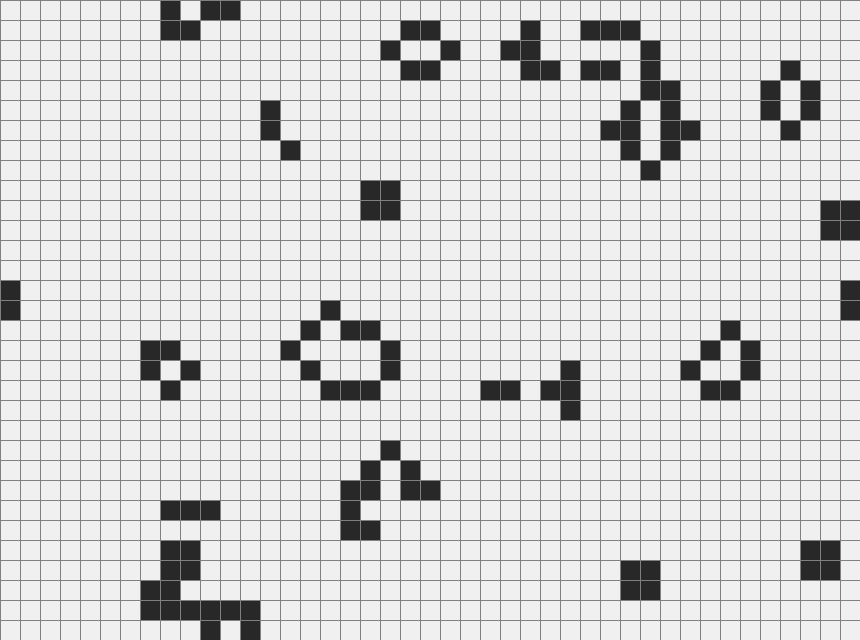
\includegraphics[scale=0.22]{figure/lifegame.png}
\end{center}
\caption{ライフゲーム\newline
{\footnotesize 黒いマスが生きたセルを表し,それぞれのセルは周囲のセルの状態によって生存・死滅が決定する.
周期的に振動するものや移動するものなど様々なパターンが現れる.}}
\label{pic_lifegame}
\end{figure}


%%% ========================================================
\subsection{基本セルオートマトン}

セルの状態が$\{0, 1\}$のいずれかをとり,次の状態が,自身と隣接する二つのセルの状態によって決定されるような一次元セルオートマトンを基本セルオートマトンと呼びます.
\footnote{特徴を列挙して,一次元二状態三近傍セルオートマトンと呼ぶこともあります.}
またここで,一次元セルオートマトンとは,セルが直線状(一次元)に配置されているようなものを指します.
\footnote{セルが平面上に配置されるライフゲームは二次元セルオートマトンです.}
この章では基本セルオートマトンについて見ていきます.


%%% ========================================================
\subsection{状態遷移とWolframコード}

基本セルオートマトンでは,あるセルの次の状態は,そのセルと隣接する二つ(左隣・右隣)のセルの現在の状態によって決定されます.
ここで,この三つのセルの現在の状態より,次の状態を決定する遷移の規則が必要となります.

いま,基本セルオートマトンを考えているので,遷移前の三つのセルの状態の組み合わせは全部で$2^3$通り存在します.
この8通りに対して,それぞれ遷移後の状態が2通りずつ存在するので,遷移の規則は全部で$2^8$通りだけ存在することになります.

この256通りの遷移規則について,それぞれに番号を割り当てることを考えます.
遷移規則は遷移後のセル状態の組み合わせによって特徴づけられるので,遷移後のセルの状態を順に並べ,その数字列を2進数として見たときの数をそれぞれの規則に割り当てることにします.

表\ref{tab_transrule_150}のような遷移規則を例として説明します.

\begin{table}[ht]
\begin{center}
\begin{tabular}{|c||c|c|c|c|c|c|c|c|} \hline
    自身と隣接するセルの状態 & 111 & 110 & 101 & 100 & 011 & 010 & 001 & 000 \\ \hline
    遷移後のセルの状態      &  1  &  0  &  0  &  1  &  0  &  1  &  1  &  0  \\ \hline
\end{tabular}
\end{center}
\caption{遷移規則(ルール150)}
\label{tab_transrule_150}
\end{table}

この遷移規則における遷移後の状態(表\ref{tab_transrule_150}下行)を,左から順に並べると$(1, 0, 0, 1, 0, 1, 1, 0)$となっています.
これを2進数とみると$1\times 2^7 + 1\times 2^4 + 1\times 2^2 + 1\times 2^1 = 150$なので,表1の遷移規則をルール150と呼びます.
この他の遷移規則についても同様にして番号を割り当てます.
このようにして割り当てられた数をWolframコードと呼びます.
\footnote{
この名前はStephen Wolframに因みます.
Stephen Wolframはセルオートマトンの解析の他に,MathmaticaやWolfram Alpha\cite{wolalp}の開発でも有名です.
}


\begin{example}
    \label{ex_transrule}
    表\ref{tab_transrule_90}のような遷移規則はルール90と呼ばれます.

    \begin{table}[ht]
    \begin{center}
    \begin{tabular}{|c||c|c|c|c|c|c|c|c|} \hline
        自身と隣接するセルの状態 & 111 & 110 & 101 & 100 & 011 & 010 & 001 & 000 \\ \hline
        遷移後のセルの状態      &  0   &  1  &  0  &  1  &  1  &  0  &  1  &  0 \\ \hline
    \end{tabular}
    \end{center}
    \caption{遷移規則(ルール90)}
    \label{tab_transrule_90}
    \end{table}
\end{example}


\begin{example}
\label{ex_update_gen}
    現在のセルの状態が\verb|"01011100"|であるような基本セルオートマトンの状態遷移を考えます.
    遷移規則はルール150として,両端は繋がっているとします.

    \begin{table}[ht]
    \begin{center}
    \begin{tabular}{|c||c|c|c|c|c|c|c|c|} \hline
        現在のセルの状態 & 0 & 1 & 0 & 1 & 1 & 1 & 0 & 0 \\ \hline
        自身と隣接するセルの状態 & 001 & 010 & 101 & 011 & 111 & 110 & 100 & 000 \\ \hline
        遷移後のセルの状態 & 1 & 1 & 0 & 0 & 1 & 0 & 1 & 0 \\ \hline
    \end{tabular}
    \end{center}
    \caption{ルール150に従う遷移計算の例}
    \label{tab_ex_update_gen}
    \end{table}

    各セルの状態遷移は表\ref{tab_ex_update_gen}のようにして計算されます.
    よって,遷移後のセルの状態は\verb|"11001010"|となります.
\end{example}


最後に遷移規則をプログラムで表すことを考えます.
ここではルール150に従った状態遷移,つまり表\ref{tab_transrule_150}を関数として実装します.
コードは図\ref{code_update}のように書けます.

\begin{figure}[ht]
\begin{center}
\begin{oframed}
\footnotesize
\begin{verbatim}
    int update(int l, int t, int r) {

        /* 三つのセルの状態を引数に取り,ルール150に従って次の状態を返す関数 */
        int[] rule150 = {0, 1, 1, 0, 1, 0, 0, 1};  // ルール150における遷移後の状態を持つ配列
        int binnum = 4*l + 2*t + 1*r;              // 三つのセルの状態の並びを二進数として見たときの数 (0...7)

        return rule150[binnum];
    }
\end{verbatim}
\end{oframed}
\end{center}
\caption{ルール150に基づく遷移を計算する関数}
\label{code_update}
\end{figure}

基本セルオートマトンでは,状態は$\{0,1\}$の二通りなので,遷移前の三つのセルの状態の並びを二進数として見ると,これは0から7の自然数になります.
よってこれを配列の添字として利用しています.
配列にはこれに対応する遷移後のセルの状態を格納します.
配列は0番目から順に格納されるので,表\ref{tab_transrule_150}下行とは逆順で数が格納されることになります.

\vspace{\baselineskip}

%%% ========================================================
\begin{question}
    \label{que_update_exp}
    引数によって遷移規則を変更できるように,関数\verb|update|を拡張してください.
    つまり,三つのセルの状態とWolframコードを引数として取り,次の状態を返す関数\verb|int update(int l, int t, int r, int wcode)|を実装してください.
    正しく実装ができていれば,第四引数に150を与えたときに図\ref{code_update}で示した関数と同じ挙動を示すはずです.
\end{question}


%%% ========================================================
\subsection{実装}

ここからは,いくつかの関数を実装して,基本セルオートマトンのプログラムを完成させます.
以降の説明において,$n$回状態遷移を行ったセルを第$n$世代のセルと呼ぶことにします.


%%% =========================================
\subsubsection{大域変数}

定義する大域変数を図\ref{code_globalvar}に示します.
セルの描画サイズを\verb|SQSIZE|として与えています.
これはセルの描画の他に,セルの個数(配列\verb|cells|の要素数)・世代数の決定で使われることになります.
また,\verb|cells|はセルの状態を保持する\verb|int|型配列です.
セルの世代更新はこの配列が持つ値の更新として行います.

\begin{figure}[ht]
\begin{center}
\begin{oframed}
\footnotesize
\begin{verbatim}
    /* 大域変数 */
    final float SQSIZE = 8.0;  // セルの描画サイズ
    int[] cells;               // セルの状態を保持する配列
\end{verbatim}
\end{oframed}
\end{center}
\caption{大域変数}
\label{code_globalvar}
\end{figure}


%%% =========================================
\subsubsection{セルの初期化}

セルの初期化を行う関数を図\ref{code_cellinit}に示します.
この関数では,セルの状態を保持する配列\verb|cells|に初期状態(第0世代の状態)を与えます.
初期状態は,中央のセルのみを1,それ以外は0としています.
また,セルの個数は,描画時に画面に入る最大の数としています.
\footnote{
    \label{fnote_display_window}
    Processingにおいて,変数\texttt{width}は表示ウィンドウの幅を保持するシステム変数です.
    また,対になるシステム変数\texttt{height}は表示ウィンドウの高さを保持します.
    いま,セルの描画サイズは\texttt{SQSIZE}で与えられているので,表示ウィンドウ(幅)に入る最大のセル個数は\texttt{(int)(width/SQSIZE)}で得られます.
    ここで,\texttt{SQSIZE}が\texttt{float}型で定義されているので,\texttt{int}型へのキャストが必要となることに注意してください.
}

\begin{figure}[ht]
\begin{center}
\begin{oframed}
\footnotesize
\begin{verbatim}
    void initCells() {

        /* セルの初期化 */
        cells = new int[(int)(width/SQSIZE)];           // 表示ウィンドウに入るだけ
        for ( int i = 0; i < cells.length; i++ ) {
            cells[i] = ( i == cells.length/2 )? 1 : 0;  // 中央のセルのみ1,それ以外は0
        }

        return ;
    }
\end{verbatim}
\end{oframed}
\end{center}
\caption{セルの初期化関数}
\label{code_cellinit}
\end{figure}


%%% =========================================
\subsubsection{世代更新}

世代更新を行う関数を図\ref{code_cellupdate}に示します.
最初に遷移前のセルの状態を配列\verb|cpcells|に保存しています.
その後,配列\verb|cpcells|が持つ値によって各セルの状態遷移を行っています.
\footnote{
    この関数では,遷移前の状態を保持しておかないと世代更新は正しく行われません.
    例えば,\texttt{i = 1}の場合で,\texttt{cells[1] = update(cells[0], cells[1], cells[2]);}とすると,
    状態遷移は添字が小さいほうから順に行われていくので,\texttt{cells[0]}は遷移後の状態を持ち,\texttt{cells[1]}の遷移が正しく行われなくなります.
}
またこのとき,両端は繋がっているとして,遷移を行っています.
これは,添字の剰余計算によって実現されます.
\footnote{
    \texttt{i = 0}の場合に添字が負数になることを防ぐために,左隣のセルの添字のみ\texttt{cells.length}を加算してから計算しています.
}

\begin{figure}[ht]
\begin{center}
\begin{oframed}
\footnotesize
\begin{verbatim}
    void updateCells() {

        /* 遷移前のセルの状態の保存 */
        int[] cpcells = new int[cells.length];      // 遷移前のセルの状態を保持する配列
        for ( int i = 0; i < cells.length; i++ ) {
            cpcells[i] = cells[i];
        }

        /* 世代更新 (全セルの状態遷移) */
        for ( int i = 0; i < cells.length; i++ ) {
            cells[i] = update(cpcells[(i-1+cells.length)%cells.length],
                              cpcells[i],
                              cpcells[(i+1)%cells.length]);
        }

        return ;
    }
\end{verbatim}
\end{oframed}
\end{center}
\caption{世代更新関数}
\label{code_cellupdate}
\end{figure}


%%% =========================================
\subsubsection{セルの描画}

セルの描画を行う関数を図\ref{code_celldraw}に示します.
この関数では,世代数\verb|gen|を引数に取り,表示ウィンドウの上から\verb|gen|行目
\footnote{
    このプログラムでは,最終的に,セルの状態を世代順に並べたものを描くので,$y$座標はそれぞれの世代数に対応した位置としています.
}
に配列\verb|cells|が持つセルの状態を描画しています.
このとき,各セルについて,状態が1であれば黒,そうでなければ(0であれば)白でセルを描いています.

\begin{figure}[ht]
\begin{center}
\begin{oframed}
\footnotesize
\begin{verbatim}
    void drawCells(int gen) {

        for ( int i = 0; i < cells.length; i++ ) {
            fill((cells[i] == 1)? 0 : 255);        // セルの状態が1ならば黒,そうでなければ白
            square(i*SQSIZE, gen*SQSIZE, SQSIZE);  // セルの描画
        }

        return ;
    }
\end{verbatim}
\end{oframed}
\end{center}
\caption{セル描画関数}
\label{code_celldraw}
\end{figure}


%%% =========================================
\subsubsection{\texttt{draw}関数}

最後に,ここまで実装してきた関数を組み立てプログラムを完成させます.
\verb|draw|関数を図\ref{code_draw}に示します.
まず始めに初期化を行い,その後,セルの描画と世代更新を第0世代から最大の世代まで繰り返し行っています.
またここで,最大の世代は表示ウィンドウを基準に設定しています.
\footnote{
    表示ウィンドウ関連については\ref{fnote_display_window}を参照してください.
}

\begin{figure}[ht]
\begin{center}
\begin{oframed}
\footnotesize
\begin{verbatim}
    void draw() {
        initCells();
        for ( int i = 0; i < height/SQSIZE; i++ ) {
            drawCells(i);
            updateCells();
        }
    }
\end{verbatim}
\end{oframed}
\end{center}
\caption{\texttt{draw}関数}
\label{code_draw}
\end{figure}

プログラム全体は\ref{code_ECA_all}節に掲載しました.
実際にはここまでのコードに加え,\verb|setup|関数が必要になりますが,セルオートマトンと直接的な関係はないため,説明は省略します.

このプログラムを実行すると図\ref{pic_eca}のような出力が得られます.

\begin{figure}[ht]
\begin{center}
    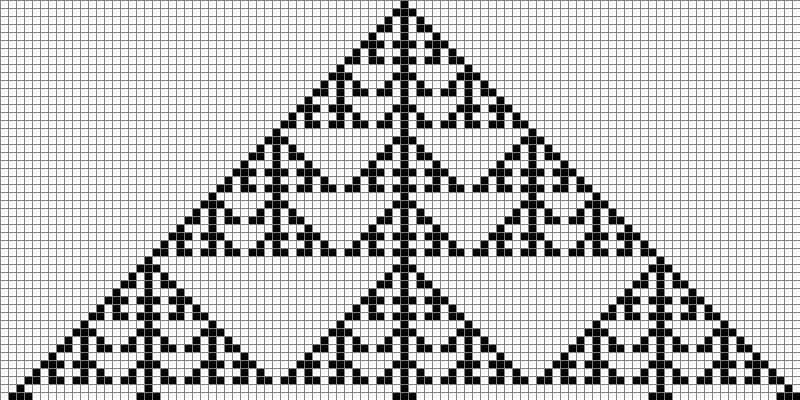
\includegraphics[scale=0.35]{figure/eca.png}
\end{center}
\caption{基本セルオートマトン(ルール150)}
\label{pic_eca}
\end{figure}


\vspace{\baselineskip}

%%% ========================================================
\begin{question}
    \label{que_cmpECA}
    この章で作成した,ルール150に従う基本セルオートマトンのプログラムに,問\ref{que_update_exp}で作成した\verb|update|関数を組み入れて,ルール150以外の規則にも対応するように拡張してください.
    作成したプログラムを実行して,ルール150以外の規則ではどのような出力が得られるのか確認してください.
    特にルール90では,どのような図形が描かれるでしょうか.
\end{question}

\begin{question}
    この章で作成した基本セルオートマトンのプログラムでは,セルの初期状態は中央のセルのみ1,それ以外は0としていました.
    この初期状態の割り当てについて,\verb|initCells|関数の\verb|for|文の内容を書き換えて,0/1がランダムに割り当てられるようにしてください.
    \href{https://processing.org/reference/random_.html}{\texttt{random}関数}が有用です.
\end{question}

\begin{question}
    ライフゲームを作成してください.
    ライフゲームは次のような規則を持ちます.
    \begin{itemize}
        \item 各セルは,生か死のいずれかの状態を持つ.
        \item あるセルの次の状態は隣接する8つのセル(左上・上・右上・左・右・左下・下・右下)の状態によって決定する.
        \item 死んでいるセルに,生きているセルがちょうど3つだけ隣接する場合,次の状態を生とする.それ以外の場合には,次の状態を死とする.
        \item 生きているセルに,生きているセルが2つまたは3つ隣接する場合,次の状態を生とする.それ以外の場合には,次の状態を死とする.
    \end{itemize}
\end{question}


%%% ========================================================
\subsection{余談: Wolfram Alpha}

最後に余談として,Wolfram Alpha\cite{wolalp}の紹介をしておきます.
Wolfram Alphaは,Wolfram Researchが開発した計算知識エンジンで,Webサービスとして公開されています.
質問に対して回答を返してくれる質問応答システムです.
面倒な計算
\footnote{
    積分計算や代数計算まで計算してくれます.
    すごい.
}
やグラフの描画なども行ってくれるので,高性能な電卓として利用できます.
計算が合わずに困ったときや,問題で与えられたの関数のグラフの概形を確かめたいといったときに利用してみると良いかもしれません.

今回取り上げた,基本セルオートマトンにも対応していて,例えば,検索窓に「ルール150」と入れると,ルール150の基本セルオートマトンの情報や基本的な性質について回答が返ってきます.
今回作成したプログラムの出力(基本セルオートマトンの世代ごとの遷移の様子)と同様の図まで懇切丁寧に出してくれます.
問\ref{que_cmpECA}の確認として利用してみてください.



%%% ============================================================================
\begin{thebibliography}{9}
    \bibitem{fractal} ケネス・ファルコナー,服部久美子(訳)「岩波科学ライブラリー291 フラクタル」岩波書店 ISBN978-4-00-029691-5 2020年
    \bibitem{fractal_1} B.マンデルブロ,広中平祐(監訳)「フラクタル幾何学 上」筑摩書房 ISBN978-4-480-09356-1 2011年
    \bibitem{fractal_2} B.マンデルブロ,広中平祐(監訳)「フラクタル幾何学 下」筑摩書房 ISBN978-4-480-09357-8 2011年
    \bibitem{chaosfractal} 山口昌哉「カオスとフラクタル」筑摩書房 ISBN978-4-480-09337-0 2010年
    \bibitem{pcweb} Processing.org (\url{https://processing.org/})
    \bibitem{genart} マット・ピアソン,久保田晃弘(監修),沖啓介(翻訳)「ジェネラティブ・アート Processingによる実践ガイド」ビー・エヌ・エヌ新社 ISBN978-4-86100-963-1 2014年
    \bibitem{cgmediaart} 近藤邦雄・田所淳(編)「ProcessingによるCGとメディアアート」講談社 ISBN978-4-06-512974-6 2018年
    \bibitem{mathgen} 巴山竜来「 数学から創るジェネラティブアート Processingで学ぶ かたちのデザイン」技術評論社 ISBN978-4-297-10463-4 2019年
    \bibitem{wolalp} Wolfram$|$Alpha (\url{https://www.wolframalpha.com/})
\end{thebibliography}



\newpage{}

%%% ============================================================================
\section{付録}

%%% ========================================================
\subsection{プログラム掲載}

本文中に登場したプログラムの全体を掲載します.
紙面の都合上,インデント形式の変更・コメントの省略など,本文中に掲載したものと体裁が異なる場合がありますが,内容面での変更はありません.


%%% ======================================
\subsubsection{Sierpinskiのカーペット}
\label{code_carpet_all}
\begin{figure}[ht]
\begin{center}
\begin{oframed}
\footnotesize
\begin{verbatim}
    /* Sierpinski carpet */

    void setup() {
        size(800, 800);   // 表示ウィンドウのサイズ設定
        background(240);  // 背景色の設定
        noLoop();         // draw関数を一度だけ実行
        noStroke();       // 図形の輪郭線なし
        fill(128);        // 図形色の設定
    }

    void draw() {
        carpet(0, 0, width, 7);
    }

    void carpet(float x, float y, float l, int n) {

        if( n <= 0 ){
            return ;
        }

        float sqlen = l / 3;  // 小正方形の辺の長さ

        square(x+sqlen, y+sqlen, sqlen);  // 中心

        carpet(x        , y        , sqlen, n-1);  // 上左
        carpet(x+sqlen  , y        , sqlen, n-1);  // 上中
        carpet(x+2*sqlen, y        , sqlen, n-1);  // 上右
        carpet(x        , y+sqlen  , sqlen, n-1);  // 中左
        carpet(x+2*sqlen, y+sqlen  , sqlen, n-1);  // 中右
        carpet(x        , y+2*sqlen, sqlen, n-1);  // 下左
        carpet(x+sqlen  , y+2*sqlen, sqlen, n-1);  // 下中
        carpet(x+2*sqlen, y+2*sqlen, sqlen, n-1);  // 下右

        return ;
    }
\end{verbatim}
\end{oframed}
\end{center}
\caption{Sierpinskiのカーペット}
\end{figure}


\newpage{}

%%% ======================================
\subsubsection{Sierpinskiのギャスケット}
\label{code_gasket_all}
\begin{figure}[ht]
\begin{center}
\begin{oframed}
\footnotesize
\begin{verbatim}
    /* Sierpinski gasket */

    void setup() {
        size(870, 760);   // 表示ウィンドウのサイズ設定
        background(240);  // 背景色の設定
        noLoop();         // draw関数を一度だけ実行
        noStroke();       // 図形の輪郭線なし
        fill(128);        // 図形色の設定
    }

    void draw() {
        float cx = width / 2;  // 三角形の中心のx座標
        float cy = 500;        // 三角形の中心のy座標
        float l = 480;         // 三角形の中心から頂点までの長さ
        gasket(cx, cy-l, cx-l*sqrt(3)/2, cy+l/2, cx+l*sqrt(3)/2, cy+l/2, 8);
    }

    void gasket(float tx, float ty, float lx, float ly, float rx, float ry, int n) {

        if ( n <= 0 ) {
            return ;
        }

        float lcx = (tx + lx) / 2;  // 上頂点と左頂点の中間点のx座標
        float lcy = (ty + ly) / 2;  // 上頂点と左頂点の中間点のy座標
        float rcx = (tx + rx) / 2;  // 上頂点と右頂点の中間点のx座標
        float rcy = (ty + ry) / 2;  // 上頂点と右頂点の中間点のy座標
        float bcx = (lx + rx) / 2;  // 左頂点と右頂点の中間点のx座標
        float bcy = (ly + ry) / 2;  // 左頂点と右頂点の中間点のy座標

        triangle(lcx, lcy, rcx, rcy, bcx, bcy);  // 中心

        gasket(tx , ty , lcx, lcy, rcx, rcy, n-1);  // 上
        gasket(lcx, lcy, lx , ly , bcx, bcy, n-1);  // 左
        gasket(rcx, rcy, bcx, bcy, rx , ry , n-1);  // 右

        return ;
    }
\end{verbatim}
\end{oframed}
\end{center}
\caption{Sierpinskiのギャスケット}
\end{figure}


\newpage{}

%%% ======================================
\subsubsection{高木曲線}
\label{code_takagi_curve_all}
\begin{figure}[ht]
\begin{center}
\begin{oframed}
\footnotesize
\begin{verbatim}
    /* Takagi curve */
    int[] ys;  // 各点の三角波の高さの和を格納する配列

    void setup() {
        size(860, 620);     // 表示ウィンドウのサイズ設定
        background(240);    // 背景色の設定
        noLoop();           // draw関数を一度だけ実行
        strokeWeight(1.6);  // 輪郭線の太さの設定
    }

    void draw() {
        reverseY();            // y軸を上向きに取る
        initPoints();          // 配列ysの初期化
        tcurve(0, width, 10);  // 高木曲線
        plot();                // 曲線のプロット
    }

    void reverseY() {
        translate(width/2, height/2);
        rotate(PI);
        translate(-width/2, -height/2);
        return ;
    }

    void initPoints() {
        ys = new int[width];
        for ( int x = 0; x < ys.length; x++ ) {
            ys[x] = 0;  // 各点の高さを0で初期化
        }
        return;
    }

    void tcurve(int lx, int rx, int n) {

        if( n <= 0 ){ return ; }

        int cx = (lx + rx) / 2;  // 区間の中心点
        int y = 0;               // 三角波の高さ

        for ( int x = lx; x < cx; x++ ) { ys[x] += y++; }
        for ( int x = cx; x < rx; x++ ) { ys[x] += y--; }

        tcurve(lx, cx, n-1);  // 左
        tcurve(cx, rx, n-1);  // 右

        return;
    }

    void plot() {
        for ( int x = 0; x < ys.length; x++ ) {
            point(x, ys[x]);
        }
        return ;
    }
\end{verbatim}
\end{oframed}
\end{center}
\caption{高木曲線}
\end{figure}


\newpage{}

%%% ======================================
\subsubsection{Koch曲線}
\label{code_koch_curve_all}
\begin{figure}[ht]
\begin{center}
\begin{oframed}
\footnotesize
\begin{verbatim}
    /* Koch curve */

    void setup() {
        size(920, 450);   // 表示ウィンドウのサイズ設定
        background(240);  // 背景色の設定
        noLoop();         // draw関数を一度だけ実行
    }

    void draw() {
        reverseY();                        // y軸を上向きに取る
        kochcurve(0, 100, width, 100, 7);  // Koch曲線
    }

    void reverseY() {

        translate(width/2, height/2);
        rotate(PI);
        translate(-width/2, -height/2);

        return ;
    }

    void kochcurve(float lx, float ly, float rx, float ry, int n) {

        if ( n <= 0 ) {
            line(lx, ly, rx, ry);
            return ;
        }

        float dx = (rx - lx) / 3;  // 小線分x成分
        float dy = (ry - ly) / 3;  // 小線分y成分
        float cx = (lx + rx) / 2;  // (lx,ly),(rx,ry)の中心x座標
        float cy = (ly + ry) / 2;  // (lx,ly),(rx,ry)の中心y座標

        kochcurve(lx             , ly             , lx+dx          , ly+dy          , n-1);  // 左
        kochcurve(lx+dx          , ly+dy          , cx-sqrt(3)/2*dy, cy+sqrt(3)/2*dx, n-1);  // 中左
        kochcurve(cx-sqrt(3)/2*dy, cy+sqrt(3)/2*dx, rx-dx          , ry-dy          , n-1);  // 中右
        kochcurve(rx-dx          , ry-dy          , rx             , ry             , n-1);  // 右

        return ;
    }
\end{verbatim}
\end{oframed}
\end{center}
\caption{Koch曲線}
\end{figure}


\newpage{}

%%% ======================================
\subsubsection{基本セルオートマトン}
\label{code_ECA_all}

\begin{figure}[ht]
\begin{center}
\begin{oframed}
\footnotesize
\begin{verbatim}
    /* Elementary Cellular Automaton */

    final float SQSIZE = 8.0;  // セルの描画サイズ
    int[] cells;               // セルの状態を保持する配列

    void setup() {
        size(800, 400);
        noLoop();
        stroke(128);
    }

    void draw() {
        initCells();
        for ( int i = 0; i < height/SQSIZE; i++ ) {
            drawCells(i);
            updateCells();
        }
    }

    void initCells() {
        cells = new int[(int)(width/SQSIZE)];           // 表示ウィンドウに入るだけ
        for ( int i = 0; i < cells.length; i++ ) {
            cells[i] = ( i == cells.length/2 )? 1 : 0;  // 中央のセルのみ1,それ以外は0
        }
        return ;
    }

    int update(int l, int t, int r) {
        int[] rule150 = {0, 1, 1, 0, 1, 0, 0, 1};  // ルール150における遷移後の状態を持つ配列
        int binnum = 4*l + 2*t + 1*r;              // 三つのセルの状態の並びを二進数として見たときの数 (0...7)

        return rule150[binnum];
    }

    void updateCells() {
        int[] cpcells = new int[cells.length];      // 遷移前のセルの状態を保持する配列
        for ( int i = 0; i < cells.length; i++ ) {
            cpcells[i] = cells[i];
        }
        for ( int i = 0; i < cells.length; i++ ) {
            cells[i] = update(cpcells[(i-1+cells.length)%cells.length],
                              cpcells[i],
                              cpcells[(i+1)%cells.length]);
        }
        return ;
    }

    void drawCells(int gen) {
        for ( int i = 0; i < cells.length; i++ ) {
            fill((cells[i] == 1)? 0 : 255);        // セルの状態が1ならば黒,そうでなければ白
            square(i*SQSIZE, gen*SQSIZE, SQSIZE);  // セルの描画
        }
        return ;
    }
\end{verbatim}
\end{oframed}
\end{center}
\caption{基本セルオートマトン(ルール150)}
\end{figure}


\newpage{}


%%% ========================================================
\subsection{その他のフラクタル}

今回は,比較的簡単に描けるフラクタル図形4つを取り上げましたが,この他にもフラクタル図形は数多く存在します.
特にMandelbrot集合(図\ref{pic_mbset})は有名なので見たことのある方も多いかと思います.

ここでは,その一部を,解説は省いて図のみの形となりますが,掲載しておきます.
興味がある方は自分の手でコードが書けるか挑戦してみてください.
以下の図は全てProcessingで描いています.


\begin{figure}[ht]
\begin{minipage}{0.5\hsize}
    \begin{center}
        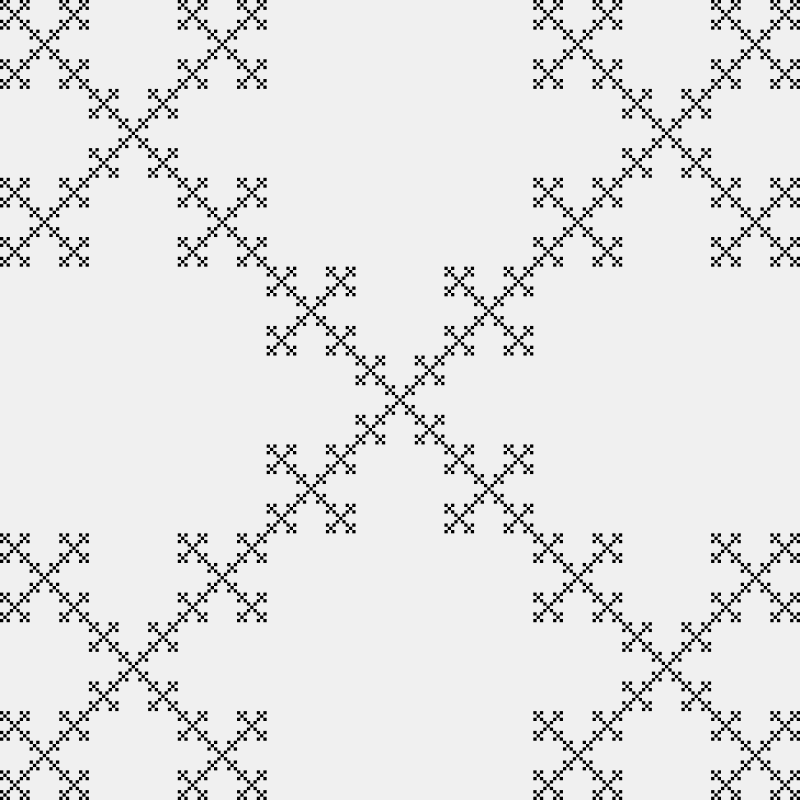
\includegraphics[scale=0.20]{figure/vicsek_fractal_saltire.png}
    \end{center}
    \caption{Vicsekフラクタル(X字)}
    \label{pic_vicfr_x}
\end{minipage}
%%%
\begin{minipage}{0.49\hsize}
    \begin{center}
        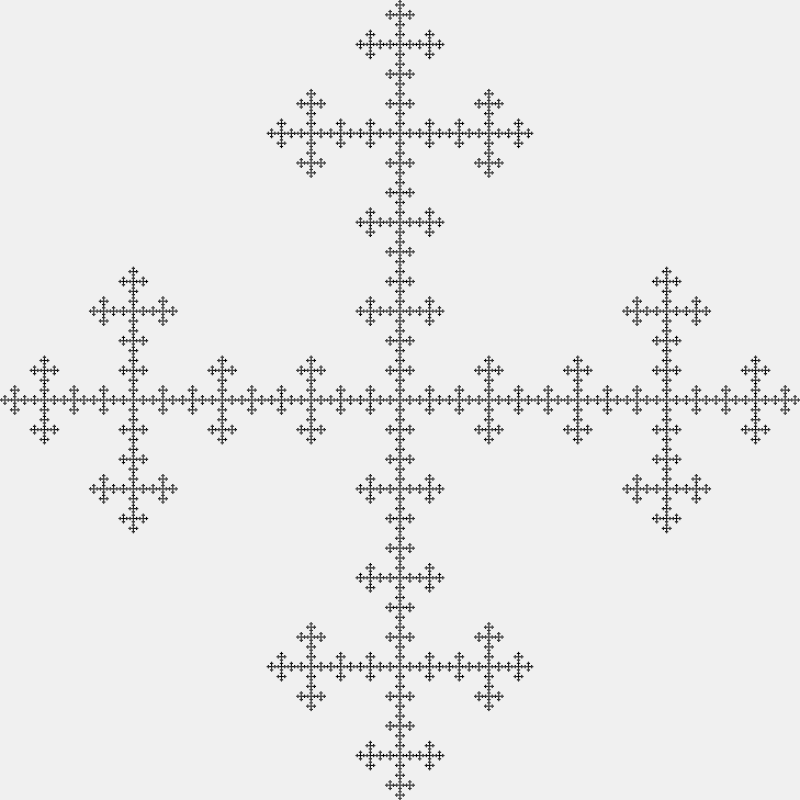
\includegraphics[scale=0.20]{figure/vicsek_fractal_cross.png}
    \end{center}
    \caption{Vicsekフラクタル(十字)}
    \label{pic_vicfr_c}
\end{minipage}
\end{figure}

\begin{figure}[ht]
\begin{minipage}{0.5\hsize}
    \begin{center}
        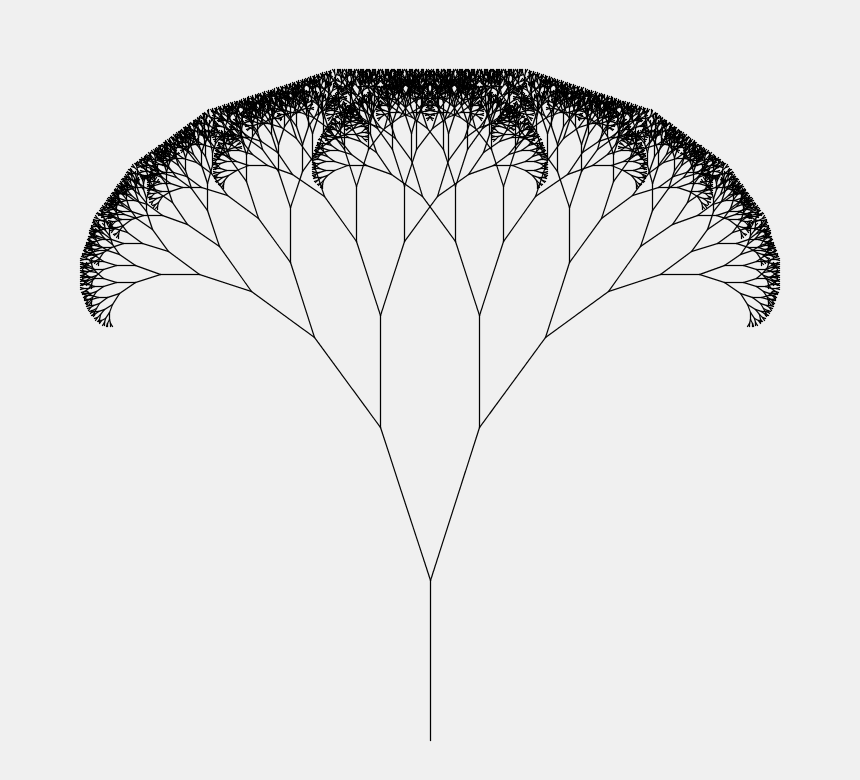
\includegraphics[scale=0.20]{figure/tree_curve.png}
    \end{center}
    \caption{樹木曲線(対称)}
\end{minipage}
%%%
\begin{minipage}{0.49\hsize}
    \begin{center}
        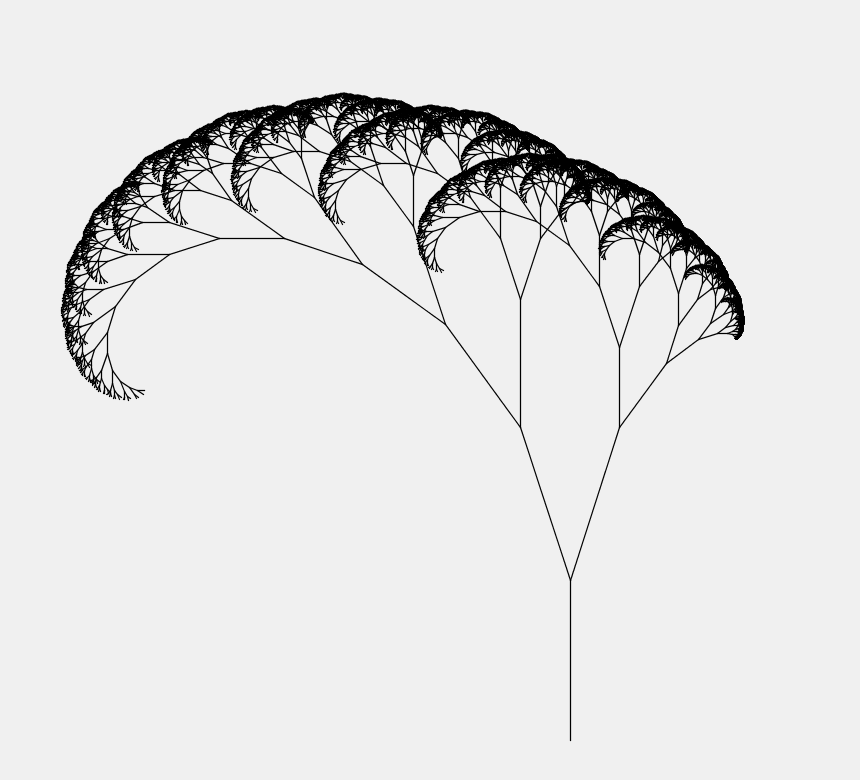
\includegraphics[scale=0.20]{figure/tree_curve_asy.png}
    \end{center}
    \caption{樹木曲線(非対称)}
\end{minipage}
\end{figure}

\begin{figure}[ht]
\begin{minipage}{0.5\hsize}
    \begin{center}
        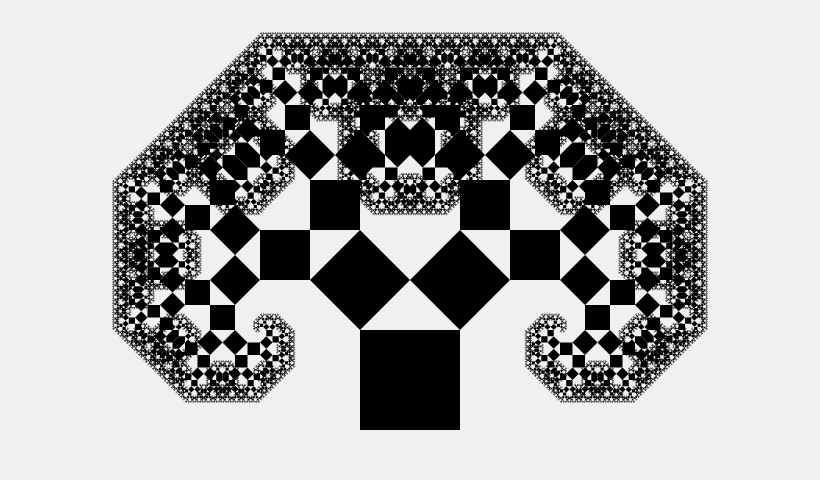
\includegraphics[scale=0.22]{figure/pythagoras_tree.png}
    \end{center}
    \caption{Pythagorasの木(対称)}
\end{minipage}
%%%
\begin{minipage}{0.49\hsize}
    \begin{center}
        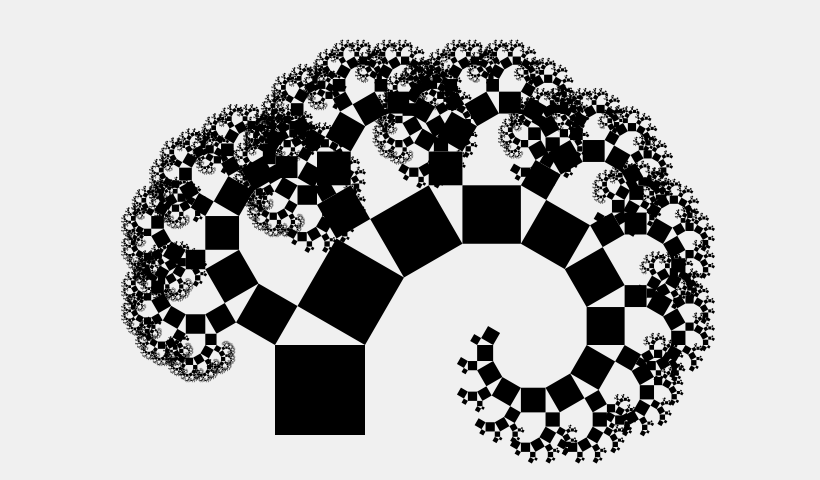
\includegraphics[scale=0.22]{figure/pythagoras_tree_asy.png}
    \end{center}
    \caption{Pythagorasの木(非対称)}
\end{minipage}
\end{figure}


\begin{figure}[ht]
\begin{minipage}{0.5\hsize}
    \begin{center}
        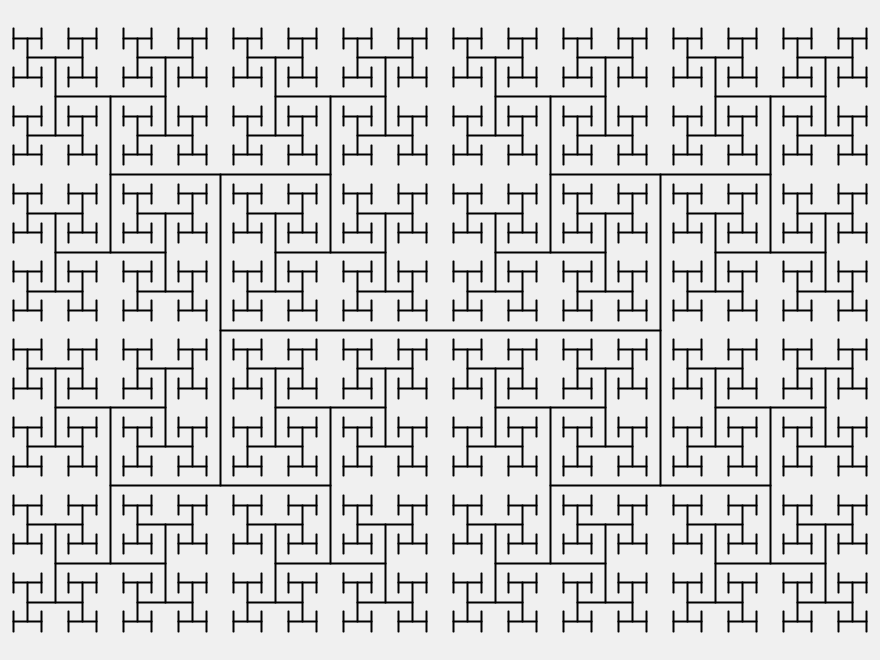
\includegraphics[scale=0.21]{figure/h_tree.png}
    \end{center}
    \caption{H木}
\end{minipage}
%%%
\begin{minipage}{0.49\hsize}
    \begin{center}
        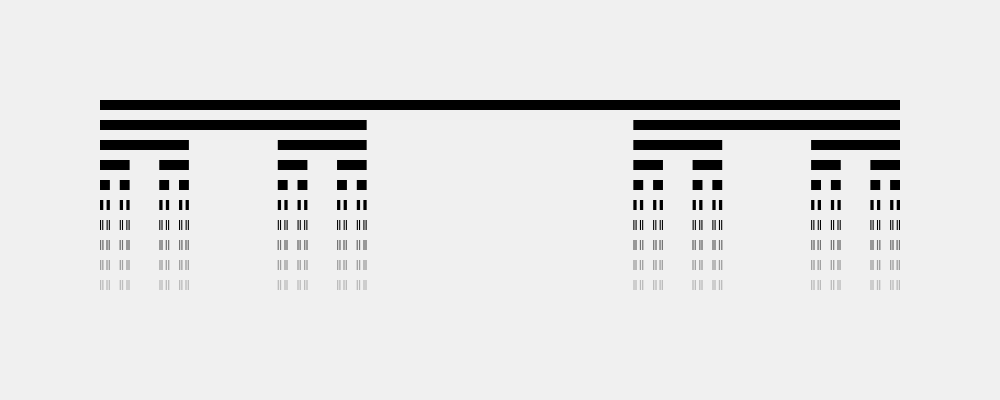
\includegraphics[scale=0.20]{figure/cantor_set.png}
    \end{center}
    \caption{Cantor集合}
    \label{pic_cantorset}
\end{minipage}
\end{figure}

\begin{figure}[ht]
\begin{minipage}{0.5\hsize}
    \begin{center}
        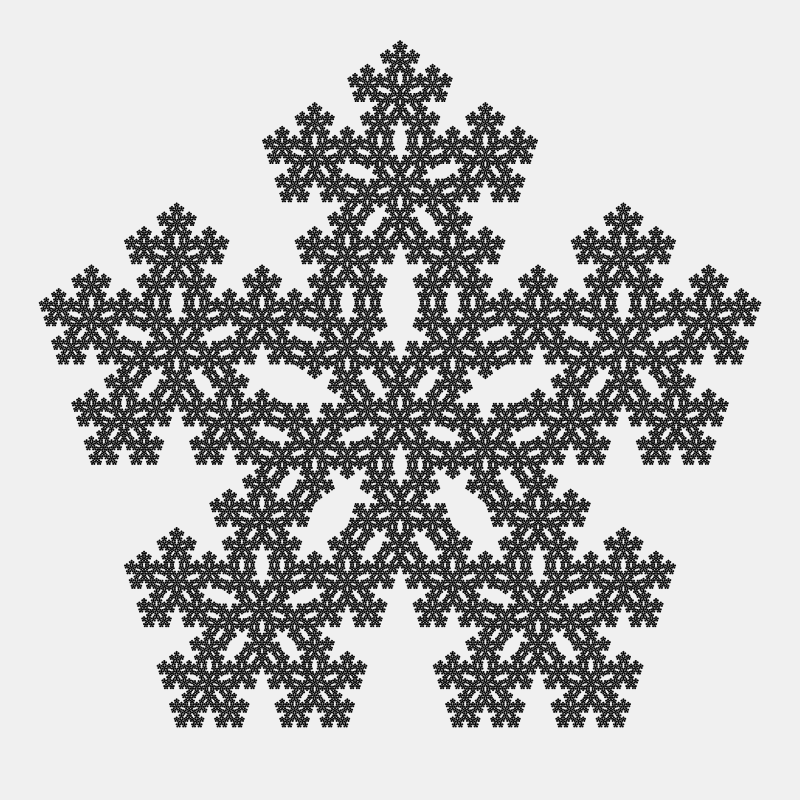
\includegraphics[scale=0.20]{figure/pentaflake.png}
    \end{center}
    \caption{Pentaflake}
\end{minipage}
%%%
\begin{minipage}{0.49\hsize}
    \begin{center}
        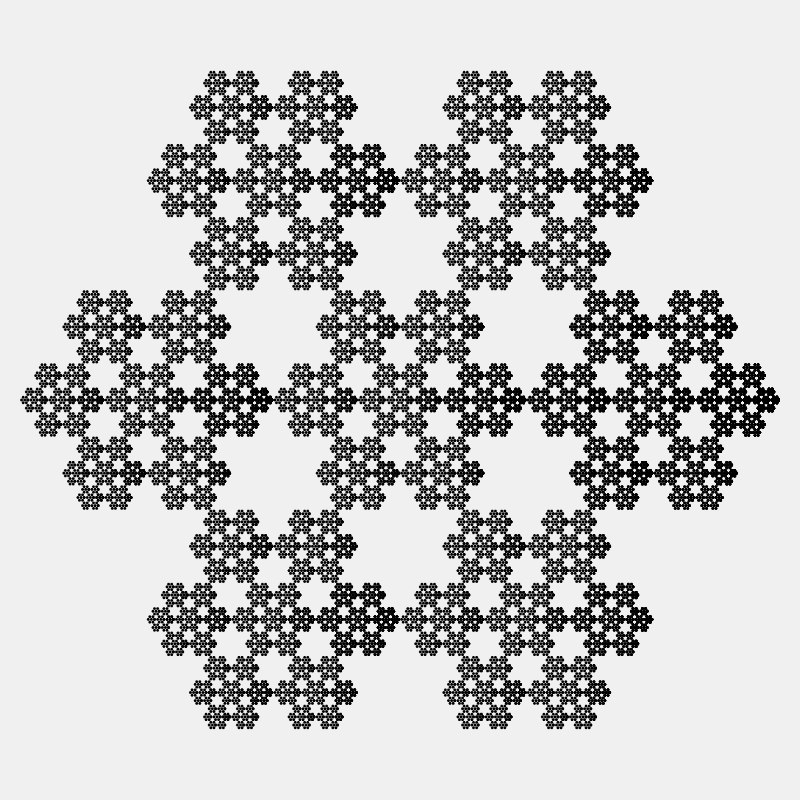
\includegraphics[scale=0.20]{figure/hexaflake.png}
    \end{center}
    \caption{Hexaflake}
    \label{pic_hexfr}
\end{minipage}
\end{figure}

\begin{figure}[ht]
\begin{minipage}{0.5\hsize}
    \begin{center}
        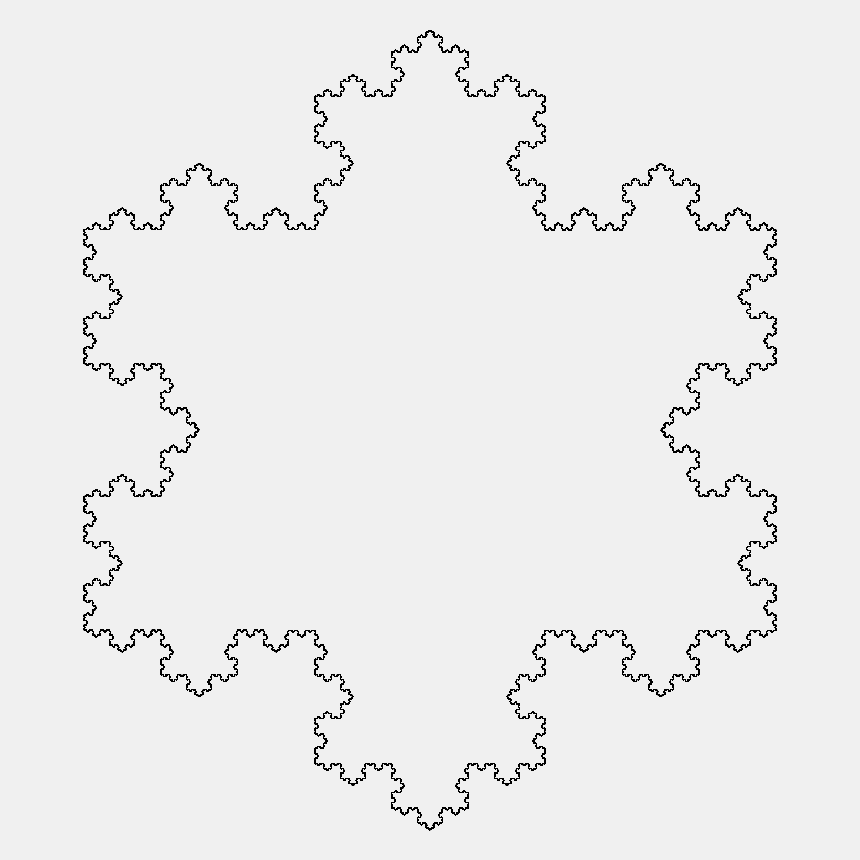
\includegraphics[scale=0.20]{figure/koch_snowflake.png}
    \end{center}
    \caption{Koch雪片}
    \label{pic_koch_snowflake}
\end{minipage}
%%%
\begin{minipage}{0.49\hsize}
    \begin{center}
        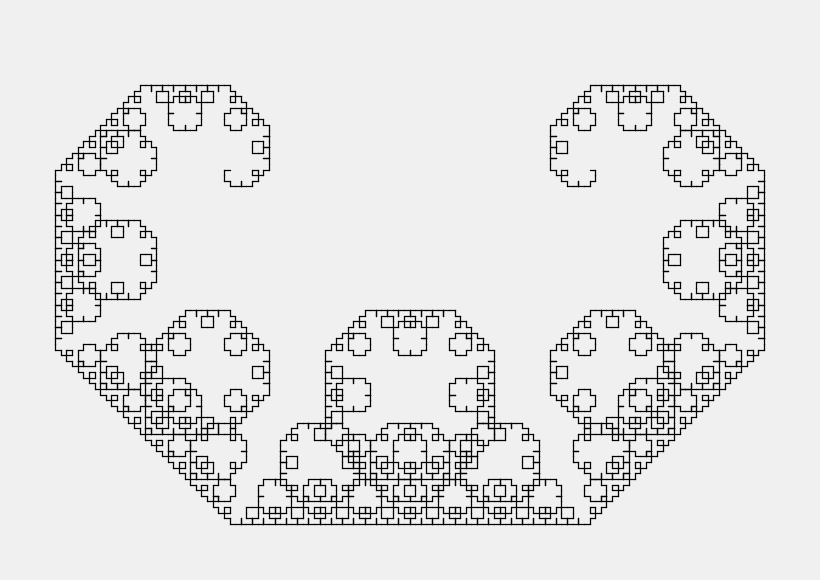
\includegraphics[scale=0.22]{figure/c_curve.png}
    \end{center}
    \caption{C曲線}
\end{minipage}
\end{figure}


\begin{figure}[ht]
\begin{minipage}{0.5\hsize}
    \begin{center}
        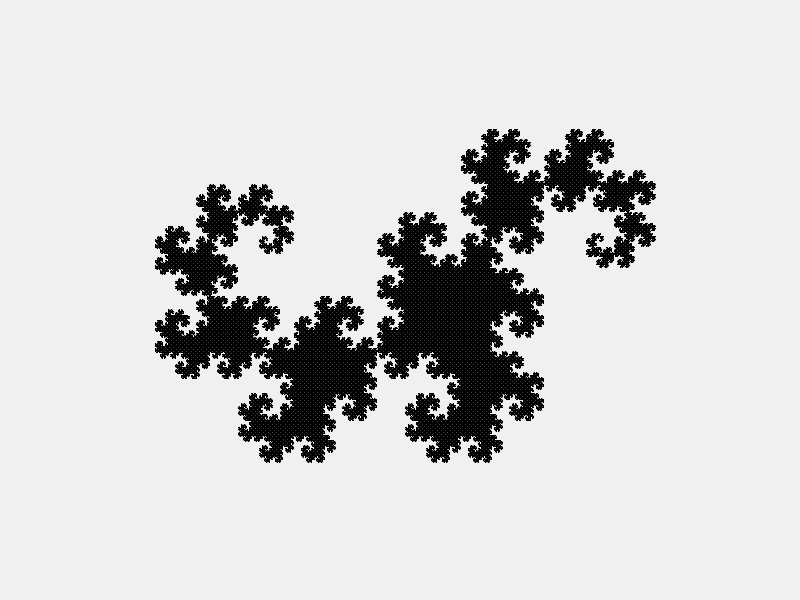
\includegraphics[scale=0.22]{figure/dragon_curve.png}
    \end{center}
    \caption{ドラゴン曲線}
\end{minipage}
%%
\begin{minipage}{0.49\hsize}
    \begin{center}
        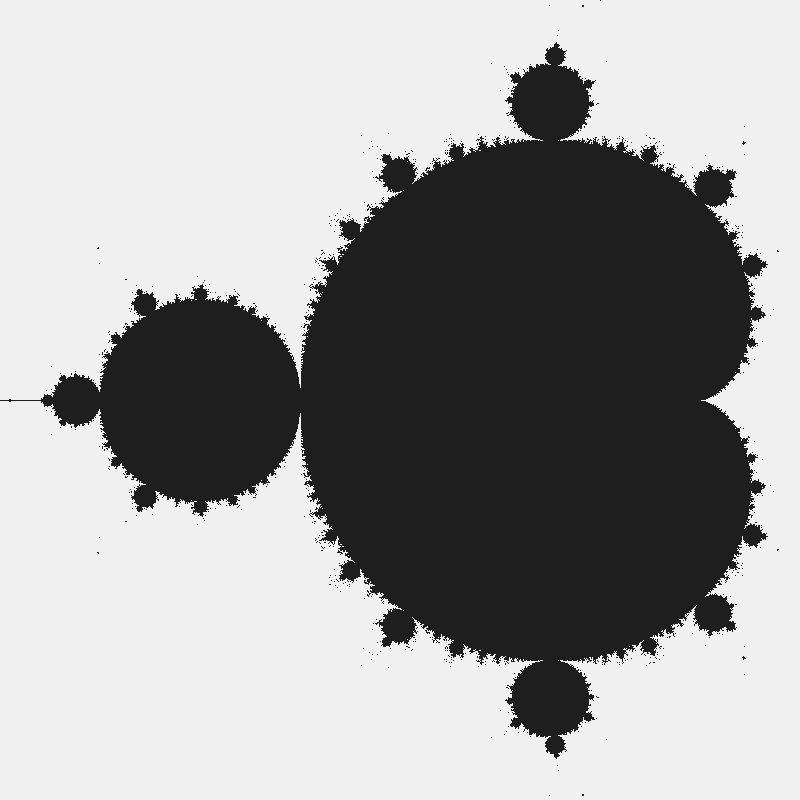
\includegraphics[scale=0.20]{figure/mandelbrot_set.png}
    \end{center}
    \caption{Mandelbrot集合}
    \label{pic_mbset}
\end{minipage}
\end{figure}

\vspace{\baselineskip}

\begin{figure}[ht]
\begin{minipage}{0.5\hsize}
    \begin{center}
        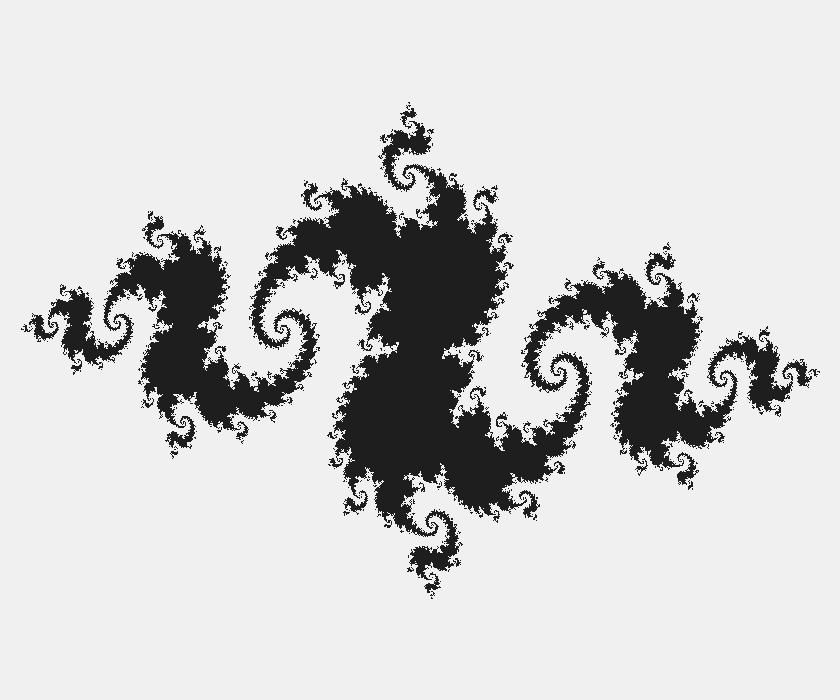
\includegraphics[scale=0.21]{figure/julia_set.png}
    \end{center}
    \caption{Julia集合(1)}
\end{minipage}
%%
\begin{minipage}{0.49\hsize}
    \begin{center}
        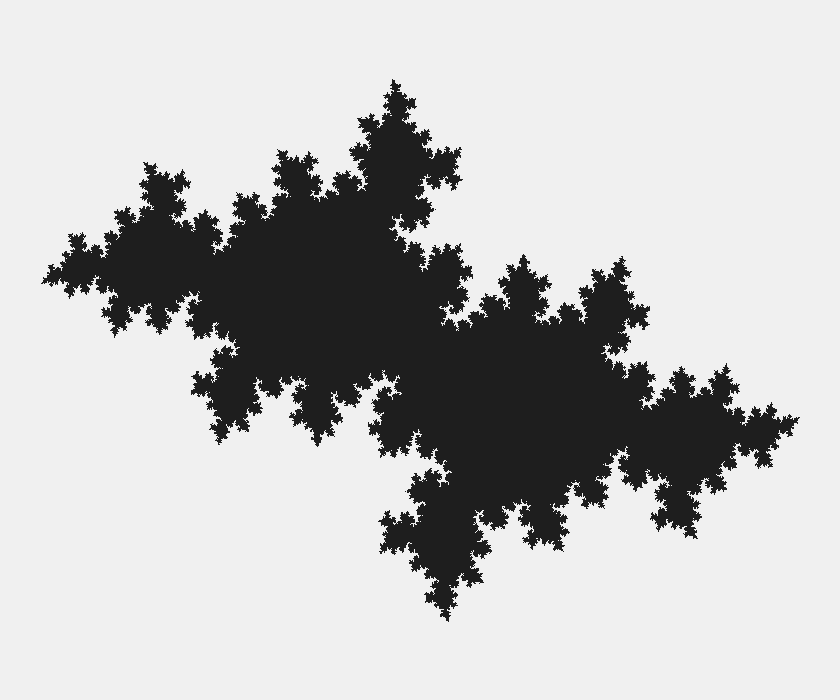
\includegraphics[scale=0.21]{figure/julia_set2.png}
    \end{center}
    \caption{Julia集合(2)}
\end{minipage}
\end{figure}

\vspace{\baselineskip}

\begin{figure}[ht]
\begin{minipage}{0.5\hsize}
    \begin{center}
        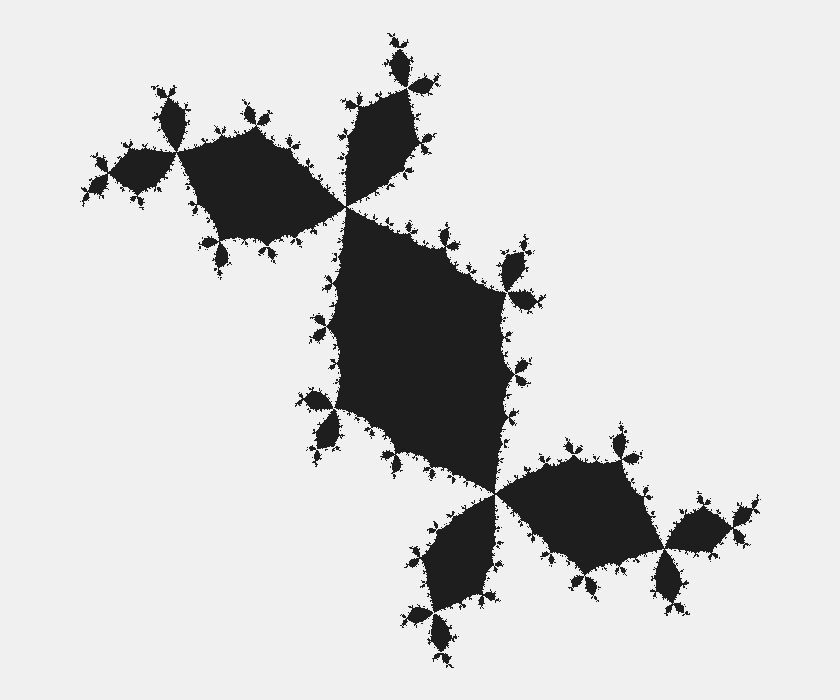
\includegraphics[scale=0.21]{figure/julia_set3.png}
    \end{center}
    \caption{Julia集合(3)}
\end{minipage}
%%
\begin{minipage}{0.49\hsize}
    \begin{center}
        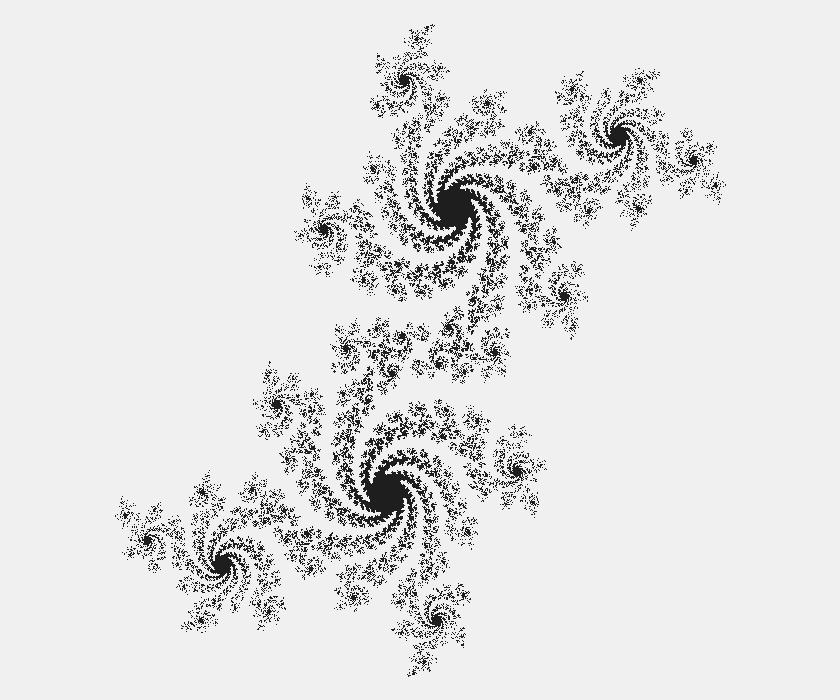
\includegraphics[scale=0.21]{figure/julia_set4.png}
    \end{center}
    \caption{Julia集合(4)}
\end{minipage}
\end{figure}


\begin{figure}[ht]
\begin{minipage}{0.5\hsize}
    \begin{center}
        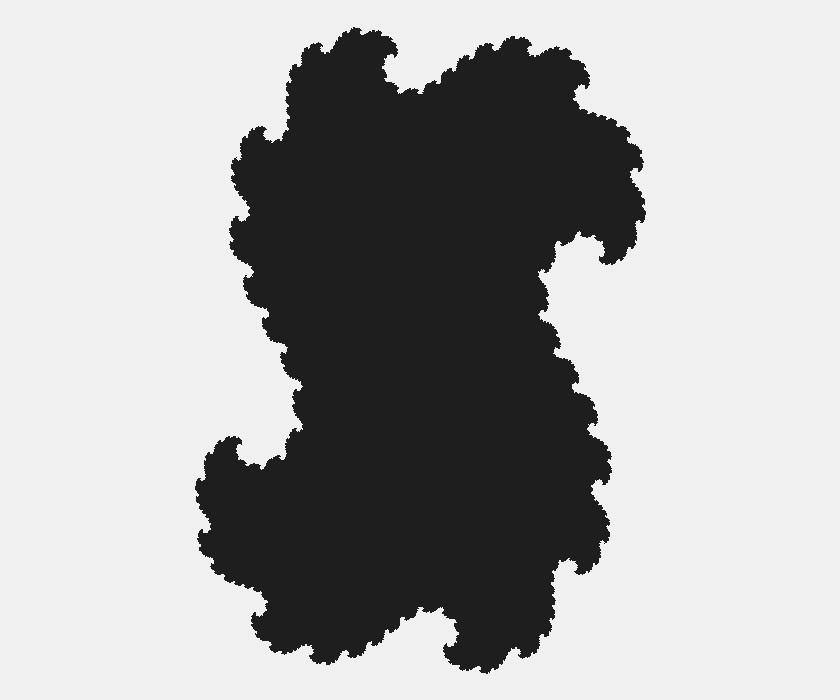
\includegraphics[scale=0.21]{figure/julia_set5.png}
    \end{center}
    \caption{Julia集合(5)}
\end{minipage}
%%
\begin{minipage}{0.49\hsize}
    \begin{center}
        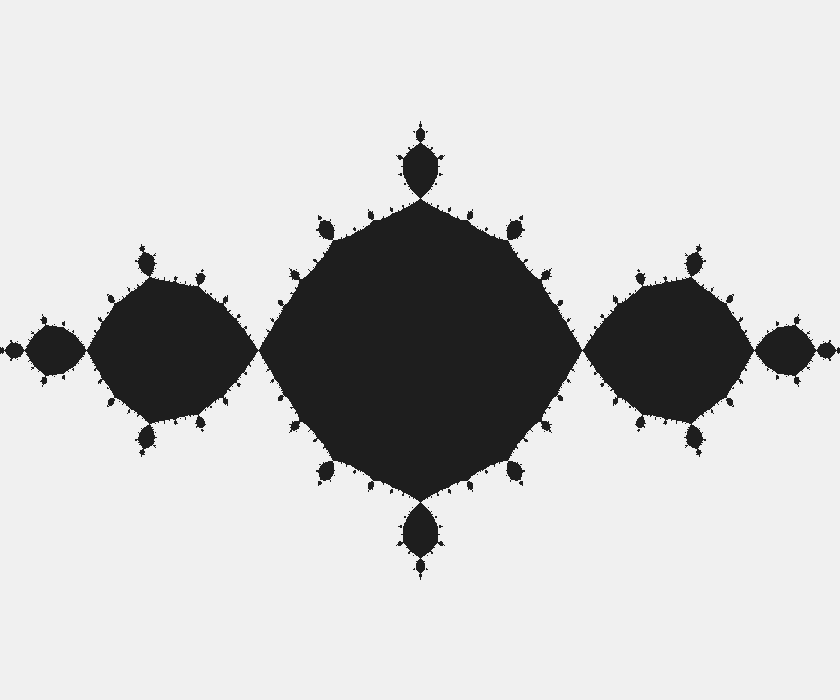
\includegraphics[scale=0.21]{figure/julia_set6.png}
    \end{center}
    \caption{Julia集合(6)}
\end{minipage}
\end{figure}

\begin{figure}[ht]
\begin{minipage}{0.5\hsize}
    \begin{center}
        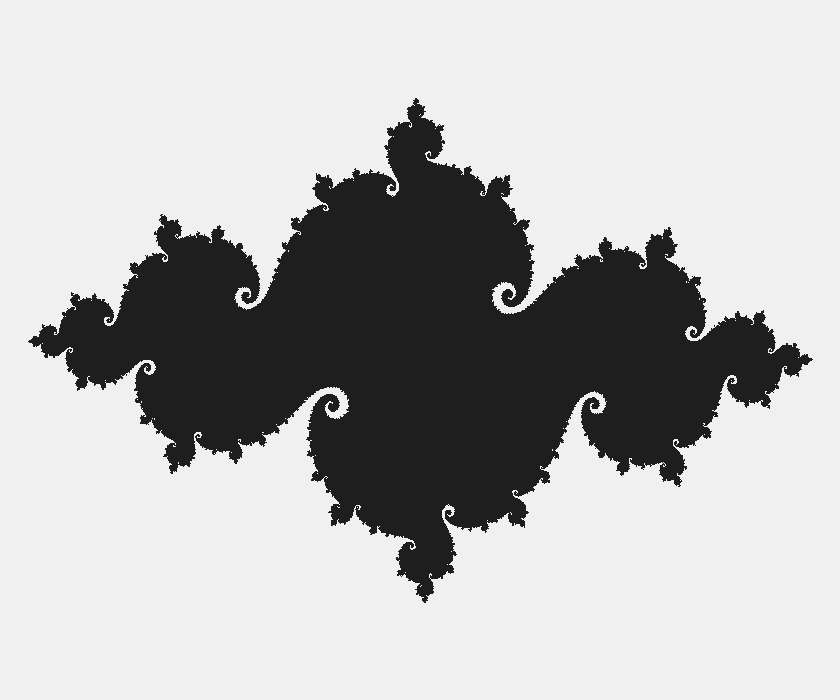
\includegraphics[scale=0.21]{figure/julia_set7.png}
    \end{center}
    \caption{Julia集合(7)}
\end{minipage}
%%
\begin{minipage}{0.49\hsize}
    \begin{center}
        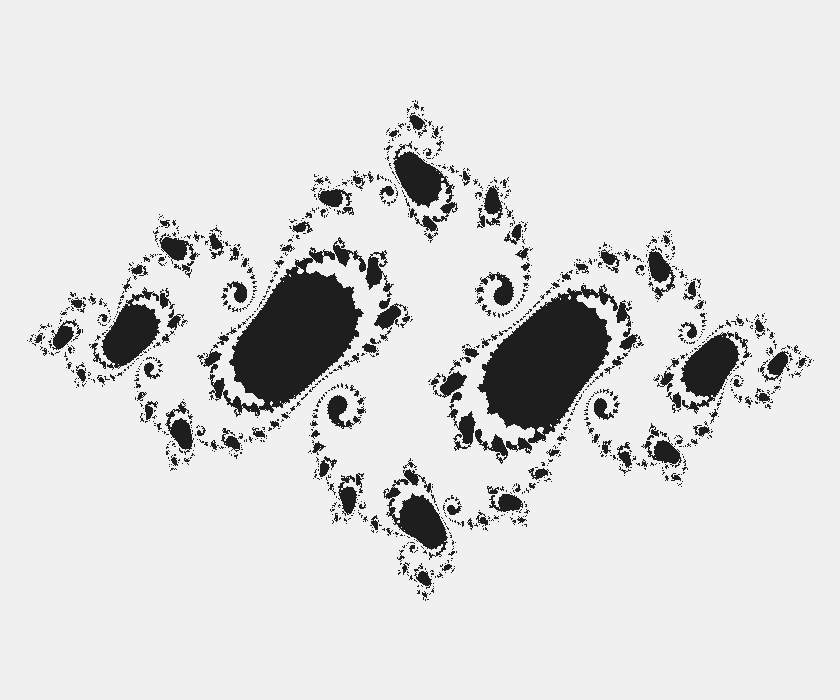
\includegraphics[scale=0.21]{figure/julia_set8.png}
    \end{center}
    \caption{Julia集合(8)}
\end{minipage}
\end{figure}

\begin{figure}[ht]
\begin{minipage}{0.5\hsize}
    \begin{center}
        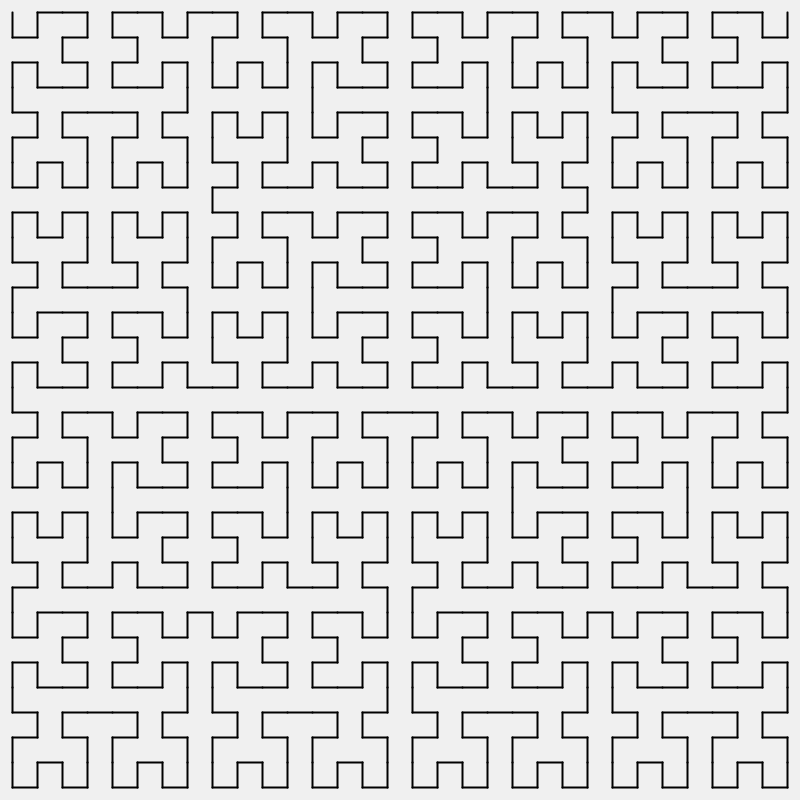
\includegraphics[scale=0.20]{figure/hilbert_curve.png}
    \end{center}
    \caption{Hilbert曲線}
\end{minipage}
%%
\begin{minipage}{0.49\hsize}
    \begin{center}
        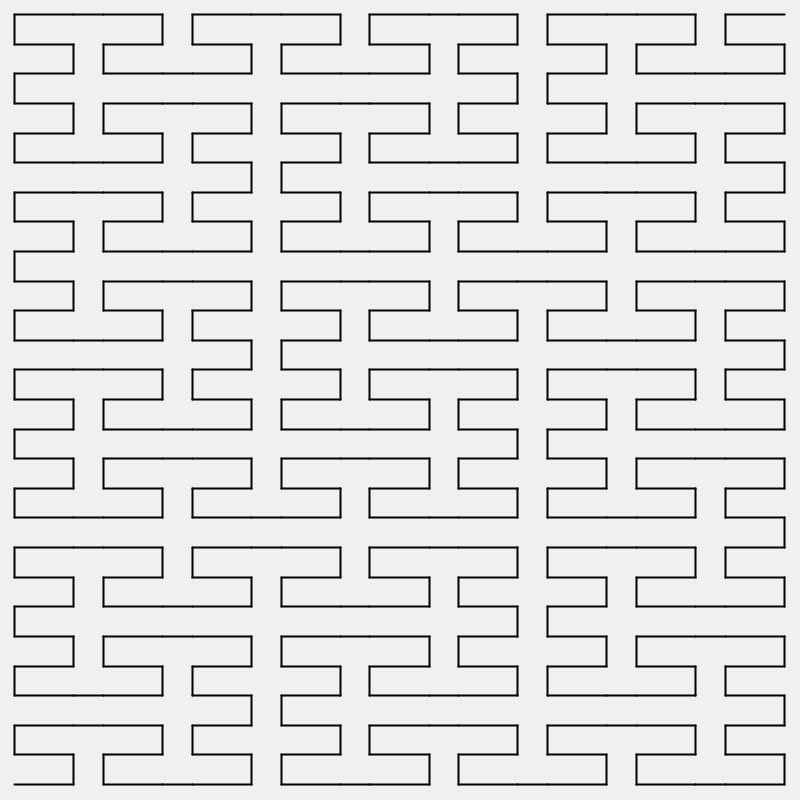
\includegraphics[scale=0.20]{figure/peano_curve.png}
    \end{center}
    \caption{Peano曲線}
\end{minipage}
\end{figure}


\end{document}
